\documentclass[11pt,leqno]{article}

\usepackage{amssymb}
\usepackage{amsmath}
\usepackage{mathrsfs}
\usepackage{xcolor}
\usepackage{mathrsfs}
\usepackage{hyperref}
\usepackage{comment}
\usepackage{graphicx}
\usepackage{indentfirst}
\graphicspath{ {./img} }

\textwidth              16 cm
\textheight             24.5  cm
\oddsidemargin          -1   cm
\evensidemargin         -1cm
\topmargin              -1 cm
\setlength{\evensidemargin}{15.5pt}
\setlength{\oddsidemargin}{2.5pt}

\pagestyle{empty}

\def\ClasaO{{\mathcal O}}

\usepackage{algpseudocode}

\title{Tema 3}
\author{Mihai Cristian-Laurentiu 2B4, Stamate Valentin 2B4}
\date{03.01.2021}

\begin{document}

\maketitle

\section*{Problema 1}
a. Vom incerca sa demonstram prin inductie in fucntie de k ca exista un cuplaj de acelasi cardinal k care expune cel putin un nod pendant al lui T.

Pentru k = 1 : T nu are un cuplaj perfect deci $|T| \geq 3$, deci exista doua cuplaje de cardinal 1, oricare dintre ele expune un nod pendant.

Pentru k = 2 : T nu are un cuplaj perfect deci $|T| \geq 5$, T are $|T|-1$ arce, astfel daca M1 satisface toate nodurile pendante, M2, format din tot doua muchii (una comuna cu M1 si o alta muchie care nu exista in M1) pe cazul minimal cu 5 noduri, nu va satisface nodrile pendante satisfacute de M1.

Pentru k = n : T nu are un cuplaj perfect deci $|T| \geq 2n+1$, T are $|T|-1$ (deoarece este arbore) arce si cuplajul are cardinal n, deci daca un cuplaj arbitrar M va satisface toate nodurile pendante, exista (cel putin) cuplajul M' care poate contine n-1 muchii din M si o muchie e $\notin M$ care nu satisface un nod pendant. Astfel in cuplajul M' de acelasi cardinal cu M expune un nod pendant.

Astfel, oricare are fi $k=|M|$ exista un alt cuplaj de acelasi cardinal care expune un nod pendant.

b. Presupuneam ca T are un cuplaj perfect M. Daca M este cuplaj perfect (are cardinal maxim) atunci acesta satureaza toate nodurile din T ( in consecinta si toate nodurile pendante). Astfel, orice cuplaj de acelasi cardinal va satisface toate nodurile(pendante) din T deoarece are acelasi cardinal cu M care este cuplaj perfect.

In mod evident, daca exista un cuplaj maximal care nu satureaza toate nodurile pendante, acesta nu satureaza toate nodurile din T (nu este cuplaj perfect). Deci un alt cuplaj de acelasi cardinal va expune cel putin un nod pendant (rezulta din a.)

Astfel, T are un cuplaj perfect daca si numai daca orice cuplaj maximal satureaza toate nodurile pendante

\section*{Problema 2} 
Algoritmul incepe prin apelul Flow(s,$C_0$), si pe masura ce se parcurg vecinii (in adancime) apelurile sunt Flow(v,min(c[uv],$\alpha$)), astfel observam ca apelurile functiei sunt realizate fie cu capacitatea curenta a arcului fie cu capacitatea ramasa din apelurile facute de stramosii nodului curent. In ceea ce priveste fluxul, acesta se completeaza dupa ce parcurgerea ( pe o ramura ) ajunge la nodul t, de exemplu arcul [xt] cu capacitatea c va avea fluxul min(c,$\alpha$). Apoi in ordine inversa parcugerii, functia returneaza valoarea maxima a fluxului pentru fiecare arc (in cazul nodurilor din care se creeaza o ramificatie, adica are cel putin 2 copii, valoarea maxima va fi suma valorilor fluxurilor din arcele catre copii). Se observa destul de usor ca frunzele care nu au arc catre t vor avea fluxul 0. Astfel daca la fiecare a apel al functiei Flow se returneaza valoarea maxima a unui flux, tabloul x va fi un flux maxim.

Algoritmul prezentat este asemanator cu o parcurgere DFS a retelei, in sensul ca pentru a putea determina fluxul maxim, se viziteaza vecinii nodului curent ( in adancime ), astfel putem spune ca algoritmul are complexitatea  $\ClasaO(n+m)$,  unde n=$|V|$ si m=$|E|$.

\section*{Problema 3} 
a.
Stim ca $|X| = r$, unde $1 \leq r < n$. 
Cum $S = X \cup \{x_1`, x_2`,...,x_{n - r}` \}$, $x_i \notin W$ atunci $|S|$ = $|X| + n - r$ = $r + n - r$ = $n$, deci $|S| = n$.
T fiind egal cu $V \setminus S$ atunci $|T|$ = $|V| - |S|$ = $2|W| - n$ = $2n - n$ = n, deci $|T| = n$.
Astfel, am demonstrat ca $|S| = |T| = n$. 

Pentru a doua parte de demostrat avem urmatoarea imagine: \\
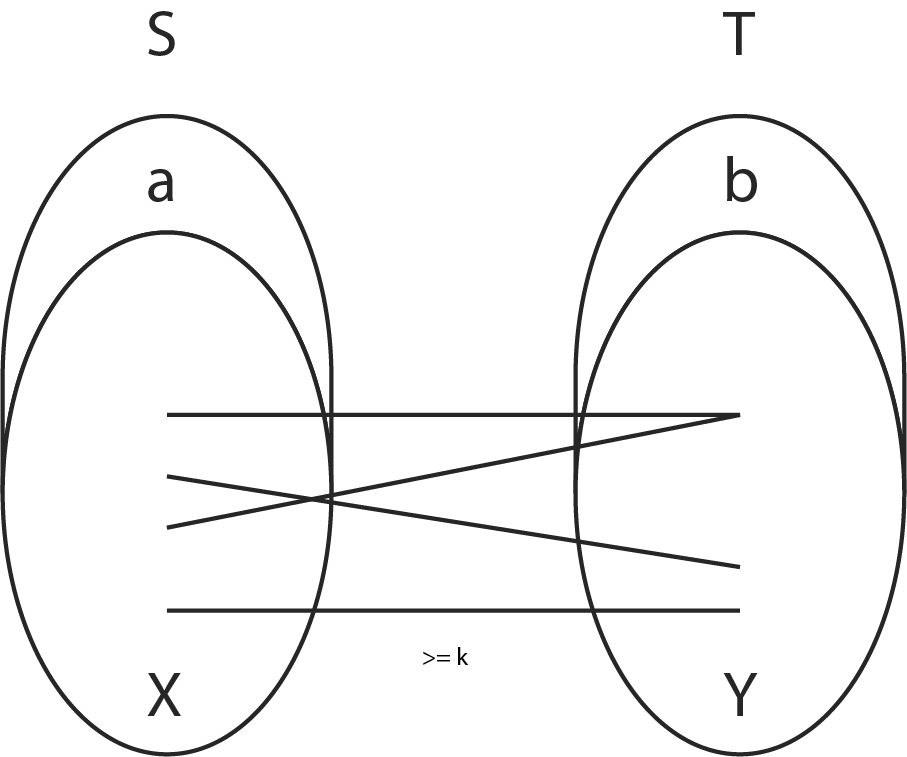
\includegraphics[width=\textwidth]{img1.jpg}

unde $a = \{x_1`, x_2`... x_{n - r}`\}$ iar $b = W` \setminus a$.
Stim ca muchiile care conecteaza $S$ si $T$ fac parte din multimea $F$.
Eliminam muchiile intre S si T, astfel nu va mai exista nici o muchie care sa le conecteze.
Mergand mai departe, unind toate celelalte moduri exceptand perichile ce fac parte din multimea F vom obtine exact multimea de muchii $E$.
Deoarece $|S| = |T| = n$, bipartitia $(S, T)$ va fi unita prin exact $n^2 - k$ deoarece $n^2$ vine de la
unirea tuturor nodurilor x, y cu $x \neq y, x \in S, y \in T$ adica $n \cdot n = n^2$ si scadem k deoarece initial avem k muchii care conecteaza S si T
dar care sunt eliminate. Astfel, am demostrat ca modulul multimii de muchii care uneste S si T este $\leq n ^2 - k$. Q.E.D

b.
Ne putem folosi de subpunctul a deoarece constructia grafului corespunde exact cu ipoteza de la acest subpunct.
Astfel, stim deja ca multimea de noduri din $X$ care face parte din $S$ este nevida datorata conditiei de la subpunctul a : $1 \leq |X| < n$.
Analog pentru Y deoarece T este obtinut din $V \setminus S$, astfel cel putin un nod din W se va afla in T. Atunci X si Y sunt nevide.
Deja cunostem faptul ca, avand desenul initial, sunt cel putin k muchii care conecteaza S si T, adica o multime de muchii care apartie subgrafului indus de W.
Atunci a doua afirmatie este adevarata, adica ceea ce aveam de demostrat.

c.
Mai intai trebuie sa demostram ca $MBC \in NP - complete$, dupa care sa reducem $simple-MAX-CUT$ la $MBC$ in tip polinomial.
Aratand cele 2 lucruri putem spune ca $MBC$ este o problema $MP-complete$.

Algorimul de mai jos rezolva problema MBC:
\begin{algorithmic}
    \State $readGraph(G, E, k)$

    \State $n = |G|$

    \State $S = ()$
    \State $nodeList = [1..n]$

    \For{$i = 1; i \leq n / 2; i++$}
        \State $node = nodeList[rand(1, nodeList.lenght)]$
        \State $nodeList.remove(node)$
        \State $S.push(node)$
    \EndFor

    \State $T = nodeList$

    \State $m = 0$
    \For{$i \in S$}
        \For{$j \in T$}
            \If{$(i, j) \in E$}
                \State $m++$
            \EndIf
        \EndFor
    \EndFor

    \If{$m \geq k$}
        \State $print("Exista \; o \; solutie")$
    \EndIf

\end{algorithmic}
Acest algoritm nedeterminist rezolva problema in timp polinomial deci ea se afla in $NP-complete$.

\section*{Problema 4} 
a. 
Un model bazat pe o retea de transport pentru a rezolva problema poate fi descris cu un graf bipartit astfel:
In prima partitie X vom avea multimea claselor iar in a doua partitie Y noua multime de clase asa cum se poate vedea in imaginea urmatoare: \\
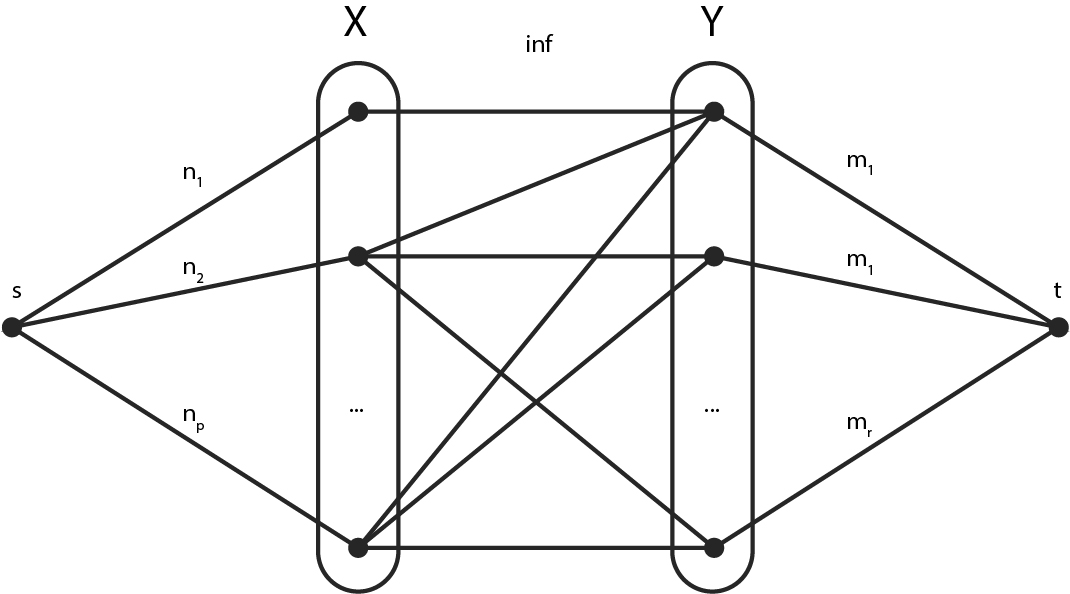
\includegraphics[width=\textwidth]{img2.jpg}

Atasam doua noduri S adiacent in mod direct cu toate nodurile din X, si T care este adiacent cu nodirile din multimea Y.
Numarul de elevi din fiecare grupa poate fi reprezentat ca si un cost pe muchia dintre nodul S si clasa curenta adica $\forall x \in X \; c_{sx} = cost(x)$ unde $cost(x)$
reprezinta numarul maxim de elevi din grupa x. Numarul de elevi al grupelor din multimea Y poate fi asociat in mod similar, costurile fiind puse pe muchiile dintre nodurile din multimea Y si nodul T.
Subgraful asociat multimii $S \cup T$ este un $K_{p,r}$ deoare vrem ca fiecare elev din grupa $x \in X$ sa poata fi redistribuit la orice grupa din $y \in Y$.
Costul este infinit deoarece suntem oricum limitati de costurile dintre multimea Y si t, astfel o noua grupa nu poate contine mai mult de c studenti din grupa veche.
Astfel am obtinut o retea de transport.

b.
Determinarea unei solutii a acestei probleme se poate rezolva aplicand un algoritm de flux maxim.
O clasa oarecare poate ceda oricati studenti incap in noua clasa. Atunci cand raman studenti, ei vor fi repartizati intr-o alta clasa. Muchiile dintre cele doua
multimi ne pot ajuta sa identific acest lucru astfel: $\forall x, y \; x \in X \; si \; y \in Y $ - "Clasa x a cedat $f_{xy}$ studenti clasei y", unde $f_{xy}$ reprezinta fluxul dintre nodurile x si y.
Aceasta modelare are solutie daca si numai daca suma consturilor asociate multimii X este egala cu suma fluxurilor asociate
multimii Y deoarece, ca sa reorganizam toti studentii in alte grupe, vom avea nevoie de acelasi numar de studenti(ca suma a studentilor noilor grupe) in noua organizare.

c. 
Pentru a determina si verifica existenta unui flux maxim pentru a acesta problema avem urmatorii algoritmi:
\begin{itemize}
    \item Algoritmul lui Ford \& Fulkerson cu etichetarea nodurilor folosing parcurgerea bfs are complexitatea $\ClasaO(n \cdot |E|^2)$. 
    Pentru verificarea exitentei solutiei la final verificam daca fluxul maxim este egal cu suma capacitatilor asociate partitiei X.
	\item Un algorim bazat pe cel precedent este cel a lui Edmonds \& Karp ce foloseste parcurgerea bfs cu o complxitatea de $\ClasaO(n \cdot |E|^2)$. Pentru verificarea solutiei se procedeaz la fel.
	\item Deoarece avem un graf bipartit putem gasi un algoritm mai eficient ce ruleaza in $\ClasaO(p \cdot r)$ ce este descris mai jos.
\end{itemize}

\pagebreak

\vspace{0.5cm}
\begin{algorithmic}
    \State $students \gets 0$
    \For{$i \in X$}
        \State $f(s, i) = c(s, i)$
        \State $students += c(s, i)$
    \EndFor

    \For {$ i \in X $}
        \For {$ j \in Y$}
            \State $ st \gets f(s, i) $
            \State $ dr \gets c(j, t) - f(j, t) $

            \State $ dr += st $
            \State $ st = 0 $
            
            \State $ f(s, i) \gets s $
            \State $ f(j, t) \gets d $
            
            \State $ b \gets d - c(j, t) $
            \If {$ b <= 0 $}
                \State $continue$
            \EndIf
 
            \State $ f(s, i) += b $
            \State $ f(j, t) \gets c(j, t) $

        \EndFor
    \EndFor
    
    $fstudents \gets 0$
    \For{$j \in Y$}
        \State $fstudents += f(s, i)$
    \EndFor

    \If{$fstudents = students$}
        \State $print("Noua \; organizare \; este \; posibila")$
    \Else
        \State $print("Noua \; organizare \; nu \; este \; posibila")$
    \EndIf


\end{algorithmic}


\end{document}
